\section{Notification functions}
\label{sec:notification_functions}
\textit{Author: Jacek Janczura} \\ \\
Notification part is a crucial part of our project as after collecting the data, preparing it and analysing it by using machine learning algorithms, we needed to find a way to communicate the results to the user. In this paragraph we will describe the motivation and ways of informing the user about the anomalies and predictions.

\subsection{Motivation}
To notify the user in order to react to main events such as anomaly detection, we created notification functions. Firstly we call the user by triggering ChatBot API. Then we send a notification to the Slack channel with a graph and a highlighted anomaly to allow the user to react faster.

\textbf{User story} \\
We decided to create a user story, where the user, who would be notified in case of an alert, is one of the administrators - Bob. Bob and his team use slack in their work, just like we do in this project. \\
In case of the anomaly detection we trigger ChatBot API to call Bob and notify him about the anomaly. To let Bob take his decision faster and - in case of an emergency - escalate the problem (or - in case of false detection - skip it), we decided to show him the graph, where he can visually assess the problem. Since Bob and his team use Slack, we decided to send them a notification to a special Slack channel as well. \\
To accelerate the decision-making process, even before logging in to the consoles, cloud watches etc. we decided to send Bob a part of the graph with the prediction and the marked anomaly. In such a way, Bob or his colleagues  receive a straightforward information of what is currently happening. The example of notification massages sent to the slack channel is depicted in a fig. \ref{fig:userNotif}.

\begin{figure}[h!]
    \centering
    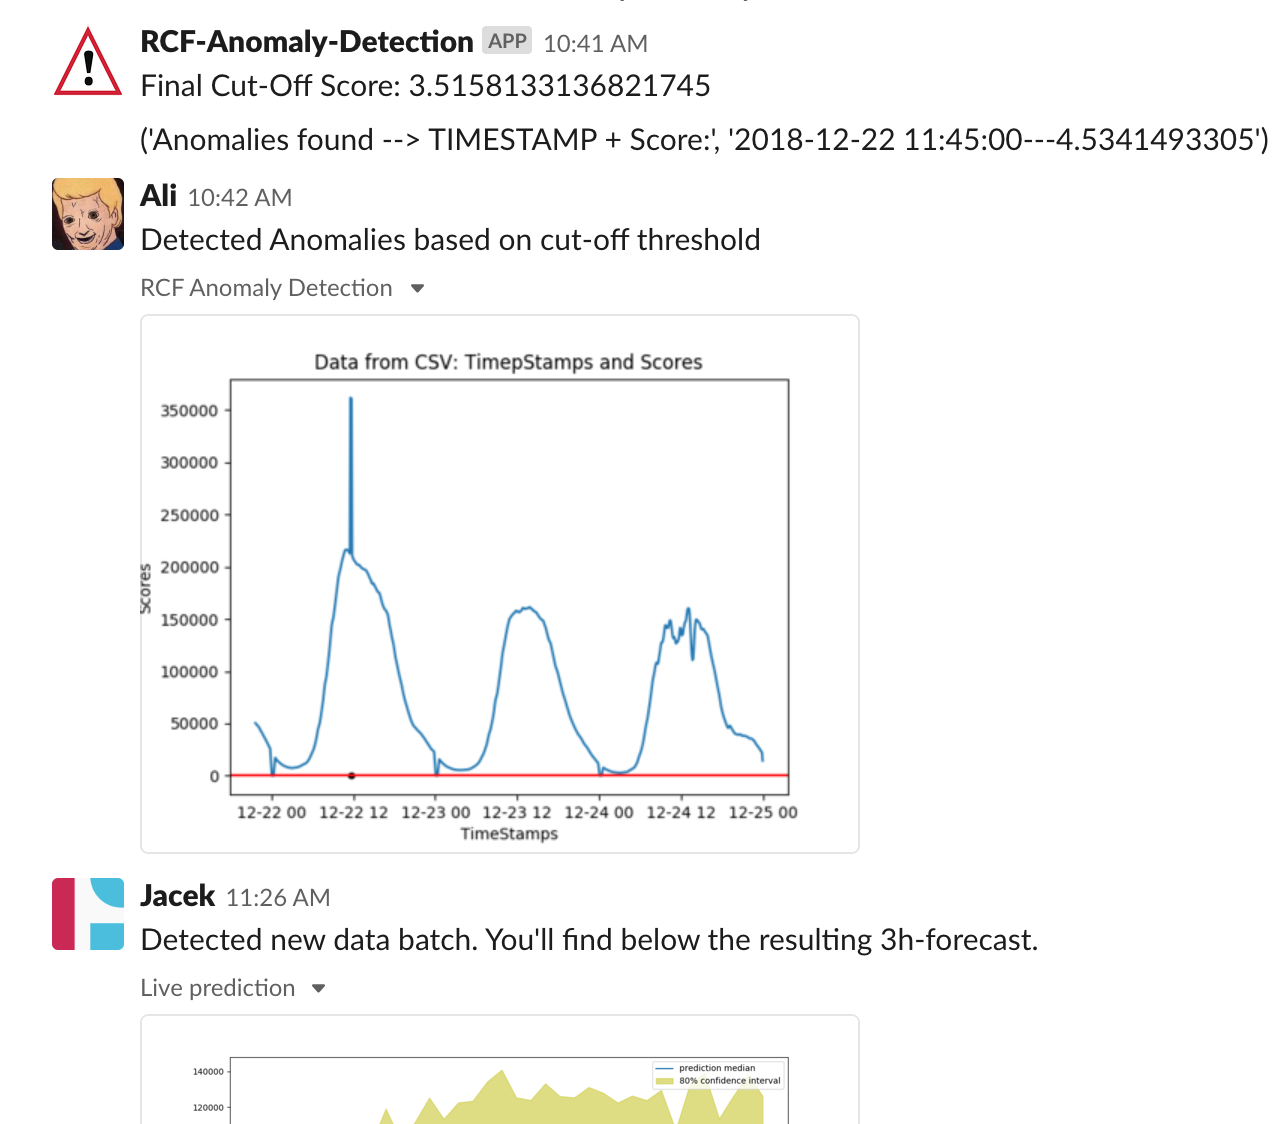
\includegraphics[width=0.75\textwidth]{images/UserNotification.png}
    \caption{Example of anomaly notification}
    \label{fig:userNotif}
\end{figure}
\newpage
\subsection{Methods to notify the user about detected anomalies}
\begin{itemize}
\item \textbf{ChatBot API notification} - To notify the ChatBot API in case of an anomaly we send REST POST message to the ChatBot API URL, as shown in an example in fig. \ref{fig:chatbot}. That POST triggers ChatBot, which calls the user.
\end{itemize}

\begin{figure}[h!]
    \centering
    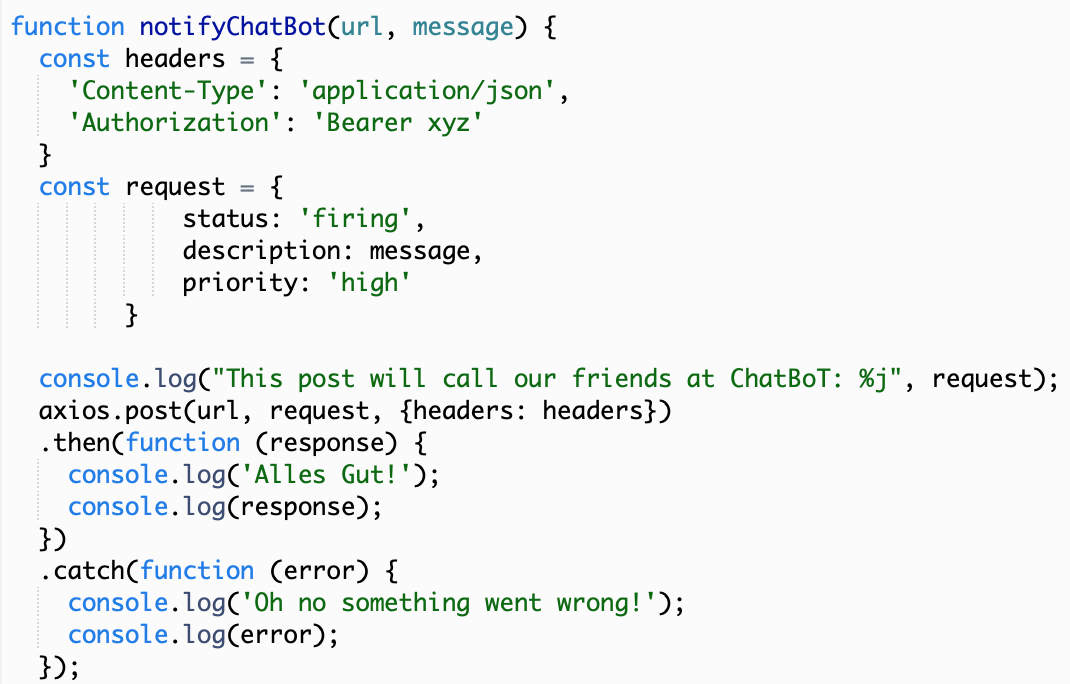
\includegraphics[width=0.8\textwidth]{images/chatbot-api-notif.png}
    \caption{Example of ChatBot API notification}
    \label{fig:chatbot}
\end{figure}


\begin{itemize}
\item \textbf{Slack channel metrics} - To inform the user about the exact metrics and data we send the message to the slack channel using Amazon Simple Notification Service topic.

\begin{lstlisting}[language=Python, caption=Sending message to slack channel using SNS topic]
    #Send Slack MSG
    sns = boto3.resource('sns')
    topic = sns.Topic('arn:aws:sns:us-east-1:746022503515:RCF-SageMaker')
    
    response = topic.publish(
        Message=str("Final Cut-Off Score: {}".format(score_cutoff)),
        Subject='#aws',
        MessageStructure='text/plain',
    )
\end{lstlisting}
\item \textbf{Slack channel graph} - Unfortunately sending the graph to the slack channel method using SNS topic did not work correctly. In order to show the graph using AWS lambda function we needed to perform the following steps:

\begin{enumerate}
\item Plot a new graph in memory.
\item Save that graph to a buffer and go to the beginning of a buffer
\begin{lstlisting}[language=Python, numbers=none]
    buf = io.BytesIO()
    plt.savefig(buf, format='png')
    buf.seek(0)
\end{lstlisting}
\item Add a buffer to a structure
\begin{lstlisting}[language=Python, numbers=none]
    my_file = {
    'file' : ('./buf.jpg', buf, 'png')}
\end{lstlisting}

\item Add that structure to the REST POST and post that file to the slack channel.

\begin{lstlisting}[language=Python, numbers=none]
    r = requests.post("https://slack.com/api/files.upload", params=payload, files=my_file)
\end{lstlisting}

\end{enumerate}
\end{itemize}

These simple notifications are an effective way to keep the user up to date with the framework.


% Amazon Simple Notification Service - to notify the easiest way.
